% ============================================================
% BAB 8 - WORKFLOW OPERASIONAL
% ============================================================

\textit{Workflow} berikut menggambarkan operasi sistem pada kondisi penggunaan
nyata. Setiap \textit{workflow} dapat dijadikan dasar \textit{test case}
\textit{end-to-end} dan \textit{smoke test} setelah perubahan fitur.

\begin{figure}[htbp]
    \centering
    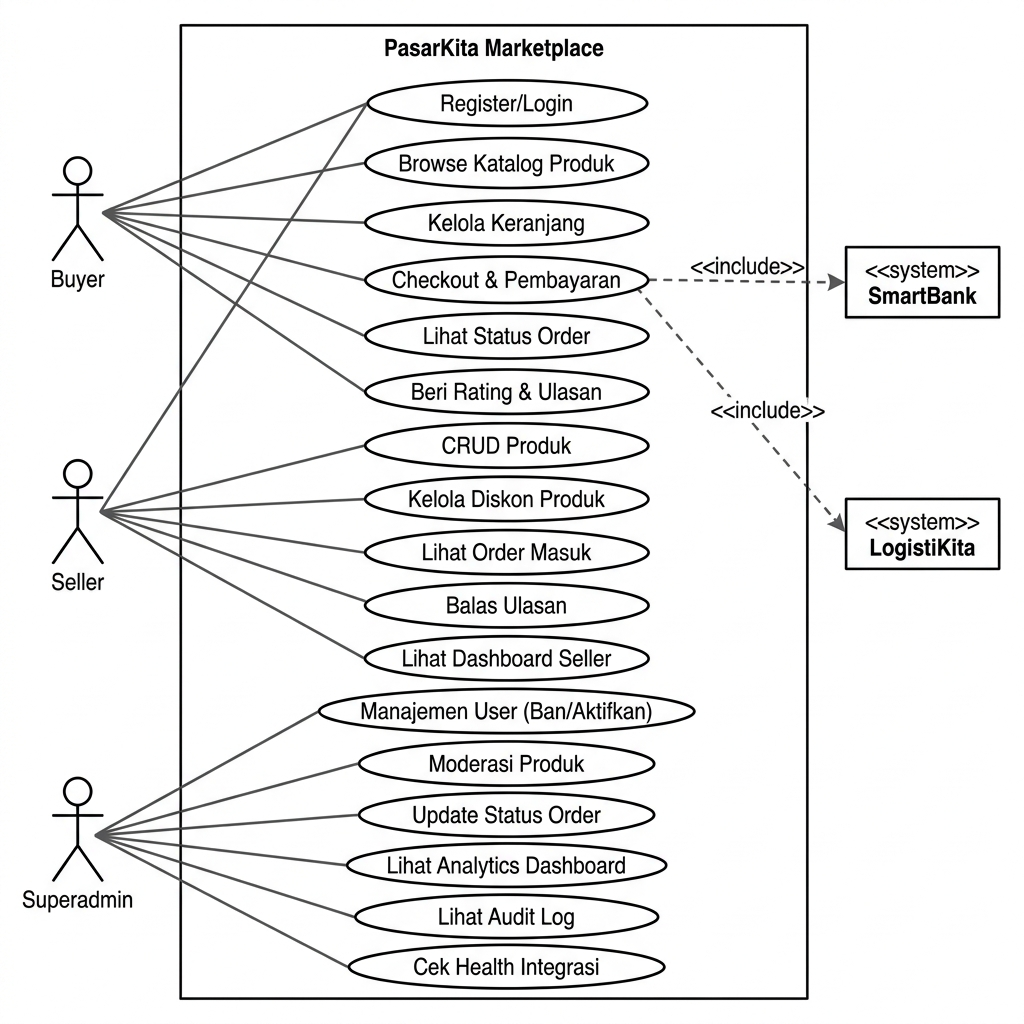
\includegraphics[width=\textwidth]{figures/usecase-diagram.png}
    \caption{Use Case Diagram Utama Sistem PasarKita}
    \label{fig:usecase-utama}
\end{figure}

\begin{longtable}{|L{2.5cm}|L{3cm}|L{5cm}|L{4cm}|}
    \caption{Workflow Operasional Utama Sistem PasarKita}
    \label{tab:workflow} \\
    \hline
    \textbf{Workflow} & \textbf{Trigger} & \textbf{Main Success Scenario}
        & \textbf{Failure / Control} \\
    \hline
    \endfirsthead
    \hline
    \textbf{Workflow} & \textbf{Trigger} & \textbf{Main Success Scenario}
        & \textbf{Failure / Control} \\
    \hline
    \endhead
    \hline
    \endfoot
    User Registration
        & \textit{User} membuka \texttt{/auth/register}.
        & Sistem memvalidasi \textit{input}, \textit{hash password}, simpan
          \textit{user}, inisiasi saldo Rp~50.000 ke SmartBank, kembalikan JWT.
        & Jika SmartBank tidak tersedia, \textit{user} tersimpan namun saldo
          belum terinisiasi; perlu \textit{retry} manual atau \textit{background
          job}. \\
    \hline
    Product Listing
        & \textit{Seller} membuka \texttt{/seller/products}.
        & \textit{Seller} membuat produk dengan \textit{form} valid; produk aktif
          dan tampil di katalog \textit{buyer}.
        & Validasi Zod gagal mengembalikan daftar \textit{field error} eksplisit;
          produk tidak tersimpan. \\
    \hline
    Checkout \& Payment
        & \textit{Buyer} menekan tombol ``Bayar'' di halaman \textit{checkout}.
        & \textit{Backend} validasi stok $\rightarrow$ kalkulasi \textit{fee}
          $\rightarrow$ buat \textit{order} pending $\rightarrow$
          \textit{payment request} ke SmartBank $\rightarrow$ \textit{update}
          \texttt{paid} $\rightarrow$ \textit{trigger} LogistiKita $\rightarrow$
          kembalikan konfirmasi.
        & Stok tidak cukup: 400 \texttt{INSUFFICIENT\_STOCK}. SmartBank gagal:
          402 \texttt{PAYMENT\_FAILED}, stok di-\textit{rollback}, \textit{order}
          \texttt{payment\_failed}. \\
    \hline
    Order Tracking
        & \textit{Buyer} membuka \texttt{/orders/:id}.
        & Sistem menampilkan status \textit{order} terkini, \texttt{tracking\_id},
          estimasi pengiriman, dan riwayat status.
        & Jika \texttt{tracking\_id} belum ada (\textit{shipping trigger} gagal),
          tampilkan status ``Menunggu Pengiriman'' dengan notifikasi admin. \\
    \hline
    Review Submission
        & \textit{Buyer} membuka detail \textit{order} dengan status
          \texttt{delivered}.
        & \textit{Buyer} mengisi \textit{rating} dan komentar; sistem memvalidasi
          status \textit{order}; \textit{rating} tersimpan; rata-rata
          \textit{rating} produk diperbarui.
        & \textit{Rating} ditolak jika \textit{order} belum \texttt{delivered}
          atau sudah pernah di-\textit{rating}; pesan \textit{error} eksplisit
          ditampilkan. \\
    \hline
    Admin User Ban
        & \textit{Superadmin} membuka \texttt{/admin/users}.
        & \textit{Superadmin} memasukkan alasan ban; sistem men-\textit{set}
          \texttt{is\_active = false}, menulis \texttt{admin\_audit\_logs}, dan
          mengembalikan status terbaru.
        & \textit{User} yang di-ban tidak dapat \textit{login}; token aktif
          \textit{user} tersebut diinvalidasi pada \textit{request} berikutnya. \\
    \hline
    Integration Health Check
        & \textit{Superadmin} membuka halaman status integrasi.
        & Sistem melakukan \textit{ping} ke API Gateway, SmartBank, dan
          LogistiKita; menampilkan status \texttt{online}/\texttt{offline} dan
          \texttt{response\_ms}.
        & Jika \textit{service} eksternal \textit{offline}, \textit{dashboard}
          tetap berjalan; status ditampilkan sebagai \texttt{offline} dengan pesan
          \textit{error} terakhir. \\
    \hline
    Analytics Pull
        & \textit{Superadmin} membuka \texttt{/admin/analytics}.
        & Sistem mengembalikan metrik agregat: total \textit{revenue},
          \textit{order count}, distribusi status, produk terlaris, dan
          \textit{revenue} per \textit{seller}.
        & Jika \textit{query timeout}, \textit{dashboard} menampilkan pesan
          \textit{error} parsial; data lain yang berhasil dimuat tetap
          ditampilkan. \\
    \hline
\end{longtable}
